\def\year{2022}\relax
%File: formatting-instructions-latex-2022.tex
%release 2022.1
\documentclass[letterpaper]{article} % DO NOT CHANGE THIS
\usepackage{aaai22}  % DO NOT CHANGE THIS
\usepackage{times}  % DO NOT CHANGE THIS
\usepackage{helvet}  % DO NOT CHANGE THIS
\usepackage{courier}  % DO NOT CHANGE THIS
\usepackage[hyphens]{url}  % DO NOT CHANGE THIS
\usepackage{graphicx} % DO NOT CHANGE THIS
\urlstyle{rm} % DO NOT CHANGE THIS
\def\UrlFont{\rm}  % DO NOT CHANGE THIS
\usepackage{natbib}  % DO NOT CHANGE THIS AND DO NOT ADD ANY OPTIONS TO IT
\usepackage{caption} % DO NOT CHANGE THIS AND DO NOT ADD ANY OPTIONS TO IT
\DeclareCaptionStyle{ruled}{labelfont=normalfont,labelsep=colon,strut=off} % DO NOT CHANGE THIS
\frenchspacing  % DO NOT CHANGE THIS
\setlength{\pdfpagewidth}{8.5in}  % DO NOT CHANGE THIS
\setlength{\pdfpageheight}{11in}  % DO NOT CHANGE THIS
%
% These are recommended to typeset algorithms but not required. See the subsubsection on algorithms. Remove them if you don't have algorithms in your paper.
\usepackage{algorithm}
\usepackage{algorithmic}

%
% These are are recommended to typeset listings but not required. See the subsubsection on listing. Remove this block if you don't have listings in your paper.
\usepackage{newfloat}
\usepackage{listings}
\lstset{%
	basicstyle={\footnotesize\ttfamily},% footnotesize acceptable for monospace
	numbers=left,numberstyle=\footnotesize,xleftmargin=2em,% show line numbers, remove this entire line if you don't want the numbers.
	aboveskip=0pt,belowskip=0pt,%
	showstringspaces=false,tabsize=2,breaklines=true}
\floatstyle{ruled}
\newfloat{listing}{tb}{lst}{}
\floatname{listing}{Listing}
%
%\nocopyright
%
% PDF Info Is REQUIRED.
% For /Title, write your title in Mixed Case.
% Don't use accents or commands. Retain the parentheses.
% For /Author, add all authors within the parentheses,
% separated by commas. No accents, special characters
% or commands are allowed.
% Keep the /TemplateVersion tag as is
\pdfinfo{
/Title (ASP-based Rule Mining)
/Author (F.~Chiariello, F.~M.~Maggi, F.~Patrizi)
/TemplateVersion (2022.1)
}

% DISALLOWED PACKAGES
% \usepackage{authblk} -- This package is specifically forbidden
% \usepackage{balance} -- This package is specifically forbidden
% \usepackage{color (if used in text)
% \usepackage{CJK} -- This package is specifically forbidden
% \usepackage{float} -- This package is specifically forbidden
% \usepackage{flushend} -- This package is specifically forbidden
% \usepackage{fontenc} -- This package is specifically forbidden
% \usepackage{fullpage} -- This package is specifically forbidden
% \usepackage{geometry} -- This package is specifically forbidden
% \usepackage{grffile} -- This package is specifically forbidden
% \usepackage{hyperref} -- This package is specifically forbidden
% \usepackage{navigator} -- This package is specifically forbidden
% (or any other package that embeds links such as navigator or hyperref)
% \indentfirst} -- This package is specifically forbidden
% \layout} -- This package is specifically forbidden
% \multicol} -- This package is specifically forbidden
% \nameref} -- This package is specifically forbidden
% \usepackage{savetrees} -- This package is specifically forbidden
% \usepackage{setspace} -- This package is specifically forbidden
% \usepackage{stfloats} -- This package is specifically forbidden
% \usepackage{tabu} -- This package is specifically forbidden
% \usepackage{titlesec} -- This package is specifically forbidden
% \usepackage{tocbibind} -- This package is specifically forbidden
% \usepackage{ulem} -- This package is specifically forbidden
% \usepackage{wrapfig} -- This package is specifically forbidden
% DISALLOWED COMMANDS
% \nocopyright -- Your paper will not be published if you use this command
% \addtolength -- This command may not be used
% \balance -- This command may not be used
% \baselinestretch -- Your paper will not be published if you use this command
% \clearpage -- No page breaks of any kind may be used for the final version of your paper
% \columnsep -- This command may not be used
% \newpage -- No page breaks of any kind may be used for the final version of your paper
% \pagebreak -- No page breaks of any kind may be used for the final version of your paperr
% \pagestyle -- This command may not be used
% \tiny -- This is not an acceptable font size.
% \vspace{- -- No negative value may be used in proximity of a caption, figure, table, section, subsection, subsubsection, or reference
% \vskip{- -- No negative value may be used to alter spacing above or below a caption, figure, table, section, subsection, subsubsection, or reference

\setcounter{secnumdepth}{1} %May be changed to 1 or 2 if section numbers are desired.

% The file aaai22.sty is the style file for AAAI Press
% proceedings, working notes, and technical reports.
%

% Title

% Your title must be in mixed case, not sentence case.
% That means all verbs (including short verbs like be, is, using,and go),
% nouns, adverbs, adjectives should be capitalized, including both words in hyphenated terms, while
% articles, conjunctions, and prepositions are lower case unless they
% directly follow a colon or long dash
\title{Technical Appendix to paper \#8198: ASP-based Declarative Process Mining}
\author{
    % Authors
% %     Francesco Chiariello,\textsuperscript{\rm 1}
% %     Fabrizio Maria Maggi, \textsuperscript{\rm 2}
% %     Fabio Patrizi \textsuperscript{\rm 1}
}
% % \affiliations{
% %     \textsuperscript{\rm 1} DIAG - Sapienza University of Rome, Italy\\
% %     \textsuperscript{\rm 2} KRDB - Free Univeristy of Bozen/Bolzano, Italy\\
% %     chiariello@diag.uniroma1.it, maggi@inf.unibz.it, patrizi@diag.uniroma1.it
% % }

%%%FP: CUSTOM PACKAGES
\usepackage{paralist}
\usepackage{xspace}
\usepackage{todonotes}
\usepackage{multirow}

\usepackage{tikz}
\usetikzlibrary{petri,arrows,backgrounds,matrix,automata,positioning,shapes,shadows,patterns,fit,calc}

\tikzset{
        ->, >=stealth, node distance=1.5cm, every state/.style={thick, minimum size = 0pt}, 
	initial text=$ $,
}

%%%%%%%%%%%%%%%%%%%%%

\input{../../macros}

\begin{document}
	\maketitle
 	%!TEX root = main.tex

\section{ASP encodings}
We report three examples of Clingo ASP programs for Log Generation,
Query Checking and Conformance Checking.

\subsection{Event Log Generation}
Consider the instance of 
Log Generation consisting of the set of 
constraints $\Phi=\{\phi_1,\phi_2\}$, with:
\begin{enumerate}
 \item $\phi_1=\always((a1 \land number<5)\limp F a2)$;
 \item $\phi_2=F (a1 \land number < 3)$.
\end{enumerate}
%%
The automaton for $\phi_1$ is depicted in Fig.~\ref{fig:response},
where:
\begin{itemize}
	\item $\varphi_1=a1 \land number<5$;
	\item $\varphi_2=a2$;
	\item $\varphi_3=\lnot \varphi_1$;
	\item $\varphi_4=\lnot\varphi_2$.
\end{itemize}
The automaton for $\phi_2$ is depicted in Fig.~\ref{fig:presence},
where:
\begin{itemize}
	\item $\varphi_1=(a1 \land number < 3)$;
	\item $\varphi_2=\lnot\varphi_1$;
	\item $\varphi_3=\true$;
\end{itemize}
%%
\begin{figure}
	\begin{center}
		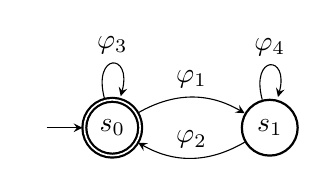
\begin{tikzpicture}
		    \node[state, initial, accepting] (s0) {$s_0$};
		    \node[state, right of=s0, xshift=.5cm] (s1) {$s_1$};
		    \draw
			(s0) edge[loop above] node{$\varphi_3$} (s0)
	            	(s0) edge[bend left, above] node{$\varphi_1$} (s1)
	            	(s1) edge[loop above] node{$\varphi_4$} (s1)
	            	(s1) edge[bend left, above] node{$\varphi_2$} (s0);
		\end{tikzpicture}
	\end{center}
\caption{Automaton for constraint $\phi_1$.\label{fig:response}}
\end{figure}
%%
\begin{figure}
	\begin{center}
		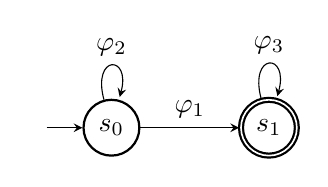
\begin{tikzpicture}
		    \node[state, initial] (s0) {$s_0$};
		    \node[state, right of=s0, xshift=.5cm, accepting] (s1) {$s_1$};
		    \draw
			(s0) edge[loop above] node{$\varphi_2$} (s0)
	            	(s0) edge[above] node{$\varphi_1$} (s1)
	            	(s1) edge[loop above] node{$\varphi_3$} (s1);
		\end{tikzpicture}
	\end{center}
\caption{Automaton for constraint $\phi_2$.\label{fig:presence}}
\end{figure}
%%
For the length of the trace(s) to return, we use the parameter 
$t$, which can be input provided when Clingo is launched.
We report the actual code for Clingo below.

\begin{small}
\begin{aspcode}
\noindent
\% PROBLEM INSTANCE\\

\noindent
\% Command~line-parameters:\\
\% t:~trace~length\\ 
(use option -c t=<value> to assign)\\

\noindent
\% Activities:\\
activity(a1).
activity(a2).
activity(a3).
activity(a4).
activity(a5).
activity(a6).
activity(a7).
activity(a8).
activity(a9).
activity(10).\\

\noindent
\% Activity attributes:\\ 
\% has\_attribute(activity, attribute name)\\
has\_attribute(a1,categorical).
has\_attribute(a1,number).\\

\noindent 
\% Attribute types:\\ 
\% value(attribute name, allowed value):\\
value(number,0..100).\\
value(categorical,c1). 
value(categorical,c2). 
value(categorical,c3).\\

\noindent
\% Automata:\\
\% Every automaton has associated a unique index\\
\% initial(automaton index, initial state)\\
\% accepting(automaton index, accepting state)\\
\% transition(automaton index, src state, 
\%~~~~~~~~~~~~~~~~~~~~formula index, dest state).\\
\% every formula has associated an index and\\
\% is associated to an automaton\\
\% (through automaton index)\\
\% holds(automaton index, formula index,\\
\%~~~~~~~~~~~~~~~~~~~~~~~~~~~~~trace index)\\

\noindent
\% phi1=G((a1 and number<5)-> F a2)\\
initial(1,s0).\\
accepting(1,s0).\\
transition(1,s0,1,s1).\\
holds(1,1,T) :- trace(a1,T),\\ 
\phantom{holds(1,1,T) :- tra}has\_value(number,V,T), V<5.
transition(1,s1,2,s0).\\
holds(1,2,T) :- trace(a2,T).\\
transition(1,s0,3,s0).\\
holds(1,3,T) :- not holds(1,1,T), time(T).\\
transition(1,s1,4,s1).\\
holds(1,4,T) :- trace(A,T), activity(A), A != a2.\\

\noindent
\% F a1 and number < 3\\
initial(2,s0).\\
accepting(2,s1).\\
transition(2,s0,1,s0).\\
holds(2,1,T) :- not holds(2,2,T), time(T).\\
transition(2,s0,2,s1).\\
holds(2,2,T) :- trace(a1,T), has\_value(number,V,T), V<3.\\
transition(2,s1,3,s1).\\
holds(2,3,T) :- time(T).\\

\noindent
\% Time points\\
time(0..t). \\

\noindent
\% PROBLEM ENCODING\\

\noindent
\% Exactly one activity per trace position\\ 
\% (0,...,t-1)\\
\{trace(A,T) : activity(A)\} = 1 :- time(T), T<t.\\

\noindent
\% Exactly one assigned value per attribute\\ 
\% associated with each activity\\
\{has\_value(K,V,T) : value(K,V)\} = 1 :- trace(A,T), has\_attribute(A,K).\\

\noindent
\% Initial state\\
cur\_state(I,S,0) :- initial(I,S).\\

\noindent
\% Transitions\\
cur\_state(I,S',T) :- cur\_state(I,S,T-1), transition(I,S,F,S'), holds(I,F,T-1).\\

\noindent
\% Trace must be accepted by all automata\\
\% Every automaton must be in at least one\\ 
\% accepting state at end of run\\
:- {cur\_state(I,S,T): not accepting(I,S), trace\_length(T)} = 0.\\

\noindent
\% Show solution\\
\#show trace/2.\\
\#show has\_value/3.\\
\end{aspcode}
\end{small}

\subsection{Query Checking}
As explained in the paper, the input of Query Checking 
includes many traces, each of which is uniquely identified by an index.
We show the input for the following two traces:
\begin{itemize}
	\item $\tau_1=a2()~a1(2,c3)~a2()$;
	\item $\tau_2=a1(2,c3)~a1(1,c2)~a1(2,c2)~a2()$,
\end{itemize}
%%
where the first attribute of activity $a1$ is named $number$ and the 
second is named $categorical$. Activity $a2$ does not contain any attribute.
We remind that since many traces are present, a further index must be added,
wrt the encoding for Log Generation, to various predicates, in order 
to indicate the trace that the predicate refers to. We denote such a predicate 
with the symbol {\asp J}.

As input constraints, we use the following event formulas with 
activity variables:
\begin{itemize}
	\item $\phi_1=\always((?A1 \land number<5) \limp F ?A2)$;
	\item $\phi_2=F (?A1 \land number < 3)$.
\end{itemize}
%%
The automaton corresponding to $\phi_1$ is depicted in Fig.~\ref{fig:response},
with: 
\begin{itemize}
	\item $\varphi_1=?A1 \land number<5$;
	\item $\varphi_2=?A2$;
	\item $\varphi_3=\lnot \varphi_1$;
	\item $\varphi_4=\lnot\varphi_2$.
\end{itemize}
%%
The automaton corresponding to $\phi_2$ is depicted in Fig.~\ref{fig:presence},
where:
\begin{itemize}
	\item $\varphi_1=(?A1 \land number < 3)$;
	\item $\varphi_2=\lnot\varphi_1$;
	\item $\varphi_3=\true$;
\end{itemize}
To account for the presence of many traces, predicate 
{\asp holds}, which models satisfaction of event formulas at
a given time point, contains an additional parameter representing 
the trace identifier. This allows to parameterize satisfaction of a 
formula wrt to the position of the trace.

Finally, as discussed in the paper, each variable $?A$ is 
modeled in the ASP program with object {\asp varA} in predicate
{\asp variable}, while the assignment to a variable {\asp varA} is 
modeled with the binary predicate {\asp assignment(varA,val)}, where 
{\asp val} is the value assigned to {\asp varA}.

The resulting encoding is shown below.\\

\begin{small}
\begin{aspcode}
\noindent
\% PROBLEM INSTANCE\\

\noindent
\% traces\\
\% trace(id,activity,position)\\

\noindent
\% tau1=a2() a1(2,c3) a2()\\
trace(1,a2,0).\\
trace(1,a1,1).\\
has\_value(1,integer,2,1).\\
has\_value(1,categorical,c3,1).\\
trace(1,a2,2).\\
trace\_length(1,3).\\

\noindent
\% tau2=a1(2,c3) a1(1,c2) a1(2,c2) a2()\\
trace(2,a1,0).\\
has\_value(2,integer,2,0).\\
has\_value(2,categorical,c3,0).\\
trace(2,a1,1).\\
has\_value(2,integer,1,1).\\
has\_value(2,categorical,c2,1).\\
trace(2,a1,2).\\
has\_value(2,integer,1,2).\\
has\_value(2,categorical,c2,2).\\
trace(2,a2,3).\\
trace\_length(2,4).\\

\noindent\% Activities\\
\% Derived from trace\\
activity(A) :- trace(\_,A,\_).\\

\noindent
\% Activity attributes:\\
\% has\_attribute(activity, attribute name)\\
has\_attribute(a1,categorical).\\
has\_attribute(a1,number).\\

\noindent
\% Attribute types:\\
\% value(attribute name, allowed value):\\
value(number,0..100).\\
value(categorical,c1).\\
value(categorical,c2).\\
value(categorical,c3).\\

\noindent
\% Automata encoding:\\
\% Almost same as Log Generation\\
\% differences: holds include trace id)\\
\% holds(automaton index, formula index,\\ 
\% \phantom{holds(au} trace id, time point)\\

\noindent
\% G((?A1 and number<5) -> F ?A2)\\
variable(varA1).\\
variable(varA2).\\
initial(1,s0).\\
accepting(1,s0).\\
transition(1,s0,1,s1).\\
holds(1,1,J,T) :- trace(J,A,T), V<5,\\ 
\phantom{ho}assignment(varA1,A), has\_value(J,integer,V,T).\\ 
transition(1,s1,2,s0).\\
holds(1,2,J,T) :- trace(J,A,T),\\ 
\phantom{holds(1,2,J,T) :- }assignment(varA2,A).\\
transition(1,s0,3,s0).\\
holds(1,3,J,T) :- not holds(1,1,J,T), time(J,T).\\
transition(1,s1,4,s1).\\
holds(1,4,J,T) :- not holds(1,2,J,T), time(J,T).\\

\noindent 
\% F ?A1 and number < 3\\
initial(2,s0).\\
accepting(2,s1).\\
transition(2,s0,1,s0).\\
holds(2,1,J,T) :- not holds(2,2,J,T), time(J,T).\\ 
transition(2,s0,2,s1).\\
holds(2,2,J,T) :- trace(J,A,T), V<3,\\ 
\phantom{ho}assignment(varA1,A), has\_value(J,integer,V,T).\\
transition(2,s1,3,s1).\\
holds(2,3,J,T) :- time(J,T).\\

\noindent
\%time points\\
time(J,0..T) :- trace\_length(J,T).\\

\noindent
\% PROBLEM ENCODING\\

\noindent
\% exactly one activity per trace point\\
\{trace(I,A,T) : activity(A)\} = 1 :- time(I,T),\\
\phantom{\{trace(I,A,T) : }T < L, trace\_length(I,L).\\

\noindent
\%initial state (J is trace identifier):\\
cur\_state(I,J,S,0) :- initial(I,S), trace(J,\_,\_).\\

\noindent
\%transitions (J is trace identifier):
cur\_state(I,J,S',T) :- cur\_state(I,J,S,T-1),\\
\phantom{cur\_state}transition(I,S,F,S'), holds(I,F,J,T-1),\\
\phantom{cur\_state}trace(J,\_,\_).\\

\noindent
\%exactly one assigned value per attribute\\
{has\_value(J,K,V,T) : value(K,V)} = 1 :- \\
\phantom{has\_value}trace(J,A,T), has\_attribute(A,K).\\

\noindent
\%exactly one assigned value per variable\\
\{assignment(Var,Val) : activity(Val)\} = 1 :- \\
\phantom{\{assignment(Var,Val)}variable(Var).\\

\noindent
:- cur\_state(I,J,S,L), trace\_length(J,L),\\
\phantom{:- }not accepting(I,S).\\

\noindent
\% solution\\
\#show trace/3.\\
\#show has\_value/4.\\
\#show assignment/2.
\end{aspcode}
\end{small}

\subsection{Conformance Checking}
As explained in the paper, this is a special case of query checking where 
the constrains are variable free, i.e., they are fully specified. 
To obtain the encoding, it is enough to replace the encoding of the automata 
with one that is fully specified, and remove the predicates related to variables, 
i.e., {\asp variable} and {\asp assignment}.
No predicates are returned as solution, as the instance is solved if the 
specification is satisfiable.

For completeness, we report the full 
ASP encoding for the set of traces used in the example of Conformance Checking 
and the constraints (automata) used for Log Generation.\\

\begin{small}
\begin{aspcode}
\noindent
\% PROBLEM INSTANCE\\

\noindent
\% traces\\
\% trace(id,activity,position)\\

\noindent
\% tau1=a2() a1(2,c3) a2()\\
trace(1,a2,0).\\
trace(1,a1,1).\\
has\_value(1,integer,2,1).\\
has\_value(1,categorical,c3,1).\\
trace(1,a2,2).\\
trace\_length(1,3).\\

\noindent
\% tau2=a1(2,c3) a1(1,c2) a1(2,c2) a2()\\
trace(2,a1,0).\\
has\_value(2,integer,2,0).\\
has\_value(2,categorical,c3,0).\\
trace(2,a1,1).\\
has\_value(2,integer,1,1).\\
has\_value(2,categorical,c2,1).\\
trace(2,a1,2).\\
has\_value(2,integer,1,2).\\
has\_value(2,categorical,c2,2).\\
trace(2,a2,3).\\
trace\_length(2,4).\\

\noindent\% Activities\\
\% Derived from trace\\
activity(A) :- trace(\_,A,\_).\\

\noindent
\% Activity attributes:\\
\% has\_attribute(activity, attribute name)\\
has\_attribute(a1,categorical).\\
has\_attribute(a1,number).\\

\noindent
\% Attribute types:\\
\% value(attribute name, allowed value):\\
value(number,0..100).\\
value(categorical,c1).\\
value(categorical,c2).\\
value(categorical,c3).\\

\noindent
\% Automata encoding:\\
\% Almost same as Log Generation\\
\% differences: holds include trace id)\\
\% holds(automaton index, formula index,\\ 
\% \phantom{holds(au} trace id, time point)\\

\noindent
\% G((a1 and number<5) -> F a2)\\
initial(1,s0).\\
accepting(1,s0).\\
transition(1,s0,1,s1).\\
holds(1,1,J,T) :- trace(J,a1,T), V<5,\\ 
\phantom{ho}, has\_value(J,integer,V,T).\\ 
transition(1,s1,2,s0).\\
holds(1,2,J,T) :- trace(J,a2,T).\\
transition(1,s0,3,s0).\\
holds(1,3,J,T) :- not holds(1,1,J,T), time(J,T).\\
transition(1,s1,4,s1).\\
holds(1,4,J,T) :- not holds(1,2,J,T), time(J,T).\\

\noindent 
\% F a1 and number < 3\\
initial(2,s0).\\
accepting(2,s1).\\
transition(2,s0,1,s0).\\
holds(2,1,J,T) :- not holds(2,2,J,T), time(J,T).\\ 
transition(2,s0,2,s1).\\
holds(2,2,J,T) :- trace(J,a1,T), V<3,\\ 
\phantom{ho}has\_value(J,integer,V,T).\\
transition(2,s1,3,s1).\\
holds(2,3,J,T) :- time(J,T).\\

\noindent
\%time points\\
time(J,0..T) :- trace\_length(J,T).\\

\noindent
\% PROBLEM ENCODING\\

\noindent
\% exactly one activity per trace point\\
\{trace(I,A,T) : activity(A)\} = 1 :- time(I,T),\\
\phantom{\{trace(I,A,T) : }T < L, trace\_length(I,L).\\

\noindent
\%initial state (J is trace identifier):\\
cur\_state(I,J,S,0) :- initial(I,S), trace(J,\_,\_).\\

\noindent
\%transitions (J is trace identifier):
cur\_state(I,J,S',T) :- cur\_state(I,J,S,T-1),\\
\phantom{cur\_state}transition(I,S,F,S'), holds(I,F,J,T-1),\\
\phantom{cur\_state}trace(J,\_,\_).\\

\noindent
\%exactly one assigned value per attribute\\
{has\_value(J,K,V,T) : value(K,V)} = 1 :- \\
\phantom{has\_value}trace(J,A,T), has\_attribute(A,K).\\

\noindent
\%exactly one assigned value per variable\\
\{assignment(Var,Val) : activity(Val)\} = 1 :- \\
\phantom{\{assignment(Var,Val)}variable(Var).\\

\noindent
:- cur\_state(I,J,S,L), trace\_length(J,L),\\
\phantom{:- }not accepting(I,S).\\

\end{aspcode}
\end{small}

	\section{File Description}

In the \emph{encodings} folder you can find the actual encoding used for the experimental evaluation. Since for comparison purposes we focus on DECLARE, the constraints are directly referred by name. The ASP-based representations of the automata corresponding to the DECLARE constraints used in the experiments are in \texttt{templates.lp}. Note that, although the encodings of the data-aware version of the problems (denoted by \texttt{\_data.lp} in the file name) can be used to solve the control-flow-only version as well in the folder is present also a simplified encoding tailored to this version.\\

In the \emph{real\_data} folder there are the 8 real dataset organized in folders. In each of them, together with the XES file there are also the discovered models in declare format and the ASP version of all such files. Note that while the models have the usual extension .lp, the log has extension .asp but is just a regular ASP file. This is done simply to make them easily recognizable and to facilitate the automation of the experiments with a script.\\

In the \emph{synth\_data} folder are present the 4 reference models used for log generation and conformance checking, together with their control-flow-only version. Note how in the latter is dealt with the local conditions to make possible to use the data-aware encoding. Again, it is possible to directly use the tailored encoding. In the folder are also present the logs of size 1000 and traces of varying length used for conformance checking and query checking. Finally, for query checking are present the files with a possible query, the relative conditions and the set of activities. File \texttt{activities.lp} needs to be used also for log generation with reference models since, being always the same, they were not included in the model itself. \\

In the \emph{utils} folder are present files with functions for performing different useful tasks, like converting from .xes and .decl to ASP files. However this has already been performed for our datasets. 
	\section{Experiment instructions}
The experiment have been performed using the ASP solver  clingo version 5.4.0. Please refer to \url{github.com/potassco/clingo} for downloading and installing clingo. \\

For executing log generation is required to pass to clingo a generation encoding file, a model file, the templates, the value of the parameter \texttt{t} corresponding to the length of the traces, and the number of desired answer sets, i.e the log size. For example you can run

\texttt{clingo generation\_encoding\_data.lp reference3\_data.lp activities.lp templates.lp -c t=10 10000}

or

\texttt{clingo generation\_encoding.lp 2012\_80.lp templates.lp -c t=10 10000}

making sure that the files are in the current directory or to pass the appropriate path. The clingo output can then be converted into an XES file (see \texttt{lp2xes.py} in \emph{utils}).\\

For executing conformance checking is required to pass to clingo a conformance encoding, a log, a model file, and the templates. For example you can run

\texttt{clingo conformance\_encoding.lp  BPI\_Challenge\_2012.asp 2012\_80.lp templates.lp}

It will return the unique answer set indicating the pairs trace/constraint such that the constraint is satisfied by the trace (and so the unsatisfied ones by exclusion).\\

For executing query checking is required to pass to clingo the query encoding, a log, a query, some conditions, the set of activities and the templates. For example you can run 

\texttt{clingo  query\_encoding\_data.lp  length\_10.lp query.lp conditions.lp activities.lp templates.lp 0}

where 0 instructs clingo to return all the assignments.


 	\section{Dataset Specifications}
While reference models and synthetic data allows to control variables like the number of constraints and the log size, and so to easily understand the different trends and how the presented approaches scale, a better grasp is also required for the real data in order to understand the effectiveness of such methods. To this end are reported here useful information about the real logs and the relative discovered models. In particular, in table \ref{tab:number_constr} are shown the number of constraints for all the models (with minimum support varying from 60 to 90) of each log and in table \ref{tab:log_specs} are shown information like the size of the logs and the average trace length. 



\begin{table}[]
\centering
\caption{Number models' constraints}
\label{tab:number_constr}
\begin{tabular}{|c|c|c|c|c|c|c|c|c|}
\hline
   & BPI2012 &   DD &     ID &    PL & PTC &   RP &     RT &    Sepsis \\ 
\hline
60 & 25   & 28 & 79 & 101 & 54   & 30 & 13 & 63 \\
\hline
70 & 25   & 29 & 73 & 72  & 41   & 30 & 10 & 35 \\
\hline
80 & 19   & 22 & 45 & 49 & 33   & 24 & 10 & 19 \\
\hline
90 & 11    &  17 & 29 & 37      & 22  &  19 & 10 & 15 \\
\hline
\end{tabular}
\end{table}

\begin{table}[h]
\centering
\caption{Logs Specifications}
\label{tab:log_specs}
\scalebox{0.6}{
\begin{tabular}{|c|c|c|c|c|c|c|c|c|}
\hline
   & BPI2012 &   DD &     ID &    PL & PTC &   RP &     RT &    Sepsis \\ 
\hline
Size & 13087 & 10500 & 6449 & 7065 & 2099 & 6886 & 150370 & 1050 \\
\hline
Activities  & 23 & 17 & 34 & 51 & 29 & 19 & 11 & 16\\
\hline
Events  & 164506 & 56437 & 72151 & 86581 & 18246 & 36796 & 561470 & 15214 \\
\hline
Min. trace len    & 3 & 1 & 3 & 3 & 1 & 1 & 2 & 3 \\
\hline
Max trace len     & 96 & 24 & 27 & 90 & 21 & 20 & 20 & 185 \\
\hline
Mean trace len    & 13 & 5 & 11 & 12 & 9 & 5 & 4 & 14\\
\hline
\end{tabular}
}
\end{table}


 	\section{Result Tables}
Finally are reported the tables for all the conducted experiments. In particular remember that for space constraints, in the paper is show only  information from the last column of tables \ref{tab:aspLogGenWData}, \ref{tab:aspLogGenWOData}, \ref{tab:alloyLogGenWData}, \ref{tab:alloyLogGenWOData}, \ref{tab:ASPLogGenReal}, \ref{tab:AlloyLogGenReal} (log generation with size 10000), and from the last column of tables \ref{tab:aspCCWData}, \ref{tab:aspCCWOData}, \ref{tab:DecAnCCWData}, \ref{tab:DecAnCCWOData} (conformance checking with synthetic data and 10 constraints).


\begin{table}[]
\caption{ASP Log generation, with data}
\label{tab:aspLogGenWData}
\scalebox{0.9}{
\begin{tabular}{|c|c|ccccccc|}
\hline
\multicolumn{2}{|c|}{Log size $\rightarrow$ }  & 100 & 250 & 500 & 1000 & 2500 & 5000 & 10000 \\
\cline{1-2}
\multicolumn{2}{|c|}{Trace len $\downarrow$ } &    &     &     &      &      &      &      \\
\hline
\hline
\multirow{5}{*}{3} &10                                         & 28 & 36  & 51  & 80 & 172 & 308 & 595    \\
&15                                                           & 33  & 47  & 70  & 114  & 240  & 457  & 876  \\
&20                                                           & 44 & 71  & 92  & 150  & 315 & 586  & 1132  \\
&25                                                           & 62  & 83  & 116 & 283  & 378  & 704  & 1364 \\
&30                                                           & 63  & 98  & 135 & 221  & 448  & 835  & 1642  \\
\hline
\hline
\multirow{5}{*}{5}&10                                         & 27  & 37  & 53 & 88 & 175 & 323 & 614   \\
&15                                                           & 38  & 56  & 76 & 121  & 249  & 474  & 894   \\
&20                                                           & 52  & 76  & 105  & 162  & 324  & 598  & 1155\\
&25                                                           & 64  & 95  & 132 & 202  & 397  & 731  & 1413\\
&30                                                           & 84  & 126  & 147 & 238  & 476  & 879  & 1701  \\
\hline
\hline
\multirow{5}{*}{7}&10                                        & 30  & 38  & 56  & 88 & 181 & 327 &  622  \\
&15                                                           & 43 & 57 & 84 & 125 & 260 & 472 & 904   \\
&20                                                           & 65 & 84 & 113 & 170 & 335 & 619 & 1178  \\
&25                                                           & 80  & 115 & 142 & 206 & 418 & 759 & 1444  \\
&30                                                           & 89  & 130 & 165 & 243 & 495 & 913 & 1746  \\
\hline
\hline
\multirow{5}{*}{10}&10                                        & 40 & 49 & 62 & 94 & 191 & 346 & 654   \\
&15                                                           & 55 & 74 & 101 & 142 & 273 & 506 & 956   \\
&20                                                           & 70 & 107 & 132 & 184 & 369 & 662 & 1250  \\
&25                                                           & 94 & 140 & 155 & 229 & 449 & 816 & 1543   \\
&30                                                           & 113 & 151 & 194 & 280 & 540 & 975 & 1874  \\
\hline 
\hline
\multicolumn{2}{|c}{ $\uparrow$ \# constraints}  &  &  &  &  &  &  &   \\
\hline
\end{tabular}
}
\end{table}

\begin{table}[]
\caption{ASP Log generation, without data}
\label{tab:aspLogGenWOData}
\scalebox{0.9}{
\begin{tabular}{|c|c|ccccccc|}
\hline
\multicolumn{2}{|c|}{Log size $\rightarrow$ }  & 100 & 250 & 500 & 1000 & 2500 & 5000 & 10000 \\
\cline{1-2}
\multicolumn{2}{|c|}{Trace len $\downarrow$ } &    &     &     &      &      &      &      \\
\hline
\hline
\multirow{5}{*}{3} &10                                                           & 10 & 14 & 21 & 35 & 76 & 137 & 249  \\
    &15                                                           & 12 & 18 & 27 & 48 & 107 & 184 & 349  \\
    &20                                                           & 14 & 21 & 33 & 55 & 119 & 232 & 436  \\
   &25                                                           & 18 & 27 & 40 & 73 & 153 & 270 & 519  \\
   & 30                                                           & 21 & 32 & 48 & 82 & 171 & 322 & 622  \\
\hline
\hline
\multirow{5}{*}{5} & 10                                                           & 11 & 17 & 22 & 35 & 77 & 141 & 270  \\
&15                                                           & 15 & 21 & 31 & 51 & 107 & 203 & 390  \\
&20                                                           & 22 & 29 & 43 & 66 & 140 & 265 & 496  \\
&25                                                           & 24 & 33 & 48 & 76 & 161 & 293 & 568  \\
&30                                                           & 33 & 38 & 58 & 96 & 194 & 349 & 666  \\

\hline
\hline
\multirow{5}{*}{7} &10                                                           & 13 & 18 & 26 & 43 & 83 & 154 & 289  \\
&15                                                           & 18 & 26 & 37 & 61 & 128 & 223 & 408  \\
&20                                                           & 24 & 32 & 45 & 72 & 150 & 278 & 538  \\
&25                                                           & 29 & 40 & 55 & 89 & 177 & 327 & 611  \\
&30                                                           & 35 & 45 & 69 & 106 & 208 & 380 & 726  \\
\hline
\hline

\multirow{5}{*}{10}&10                                                           & 18 & 22 & 32 & 50 & 102 & 181 & 340  \\
&15                                                           & 24 & 34 & 51 & 76 & 138 & 248 & 457  \\
&20                                                           & 31 & 41 & 59 & 88 & 176 & 317 & 601  \\
&25                                                           & 38 & 52 & 75 & 110 & 218 & 381 & 712  \\
&30                                                           & 49 & 61 & 87 & 131 & 255 & 450 & 837  \\
\hline 
\hline
\multicolumn{2}{|c}{ $\uparrow$ \# constraints}  &  &  &  &  &  &  &   \\
\hline 

\end{tabular}
}
\end{table}

\begin{table}[]
\caption{Alloy Log generation, with data}
\label{tab:alloyLogGenWData}
\scalebox{0.8}{
\begin{tabular}{|c|c|ccccccc|}
\hline
\multicolumn{2}{|c|}{Log size $\rightarrow$ }  & 100 & 250 & 500 & 1000 & 2500 & 5000 & 10000 \\
\cline{1-2}
\multicolumn{2}{|c|}{Trace len $\downarrow$ } &    &     &     &      &      &      &      \\
\hline
\hline
\multirow{5}{*}{3}&10                                                           & 1568 & 2408 & 3544 & 5377 & 10226 & 19082 & 35975\\
&15                                                           & 1866 & 3058 & 4624 & 7035 & 13806 & 26182 & 50649\\
&20                                                           & 2432 & 3837 & 5633 & 8839 & 19222 & 35286 & 69608  \\
&25                                                           & 2839 & 4407 & 6490 & 10559 & 23713 & 43606 & 85127  \\
&30                                                           & 3255 & 5020 & 7489 & 12029 & 26772 & 51534 & 101518  \\
\hline
\hline
\multirow{5}{*}{5}&10                                                           & 1551 & 2430 & 3585 & 5418 & 10485 & 19017 & 35786  \\
&15                                                           & 1977 & 3159 & 4766 & 7388 & 14509 & 27222 & 51534  \\
&20                                                           & 2554 & 4088 & 5966 & 9240 & 19564 & 35668 & 70342  \\
&25                                                           & 3033 & 4551 & 6653 & 10810 & 23273 & 43721 & 85598  \\
&30                                                           & 3695 & 5059 & 7570 & 12071 & 26943 & 51280 & 101882 \\
\hline
\hline
\multirow{5}{*}{7}&10                                                           & 1578 & 2492 & 3632 & 5582 & 10880 & 19395 & 36464  \\
&15                                                           & 2019 & 3323 & 4861 & 7486 & 14749 & 27452 & 54402  \\
&20                                                           & 2710 & 4242 & 6012 & 9314 & 19657 & 36552 & 73122  \\
&25                                                           & 3168 & 4573 & 6721 & 10876 & 23258 & 45096 & 87065  \\
&30                                                           & 3793 & 5275 & 7707 & 12627 & 27942 & 52492 & 106062  \\
\hline
\hline
\multirow{5}{*}{10}&10                                                           & 1636 & 2524 & 3697 & 5662 & 10673 & 20492 & 37688 \\
&15                                                           & 2221 & 3443 & 4999 & 7803 & 15893 & 28515 & 54749  \\
&20                                                           & 2764 & 4205 & 6151 & 9594 & 20393 & 37987 & 73222  \\
&25                                                           & 3333 & 4938 & 6987 & 11207 & 24102 & 45570 & 89210  \\
&30                                                           & 4027 & 5575 & 8127 & 13144 & 28890 & 54214 & 107520  \\
\hline 
\hline
\multicolumn{2}{|c}{ $\uparrow$ \# constraints}  &  &  &  &  &  &  &   \\
\hline
\end{tabular}
}
\end{table}

\begin{table}[]
\caption{Alloy Log generation, without data}
\label{tab:alloyLogGenWOData}
\scalebox{0.8}{
\begin{tabular}{|c|c|ccccccc|}
\hline
\multicolumn{2}{|c|}{Log size $\rightarrow$ }  & 100 & 250 & 500 & 1000 & 2500 & 5000 & 10000 \\
\cline{1-2}
\multicolumn{2}{|c|}{Trace len $\downarrow$ } &    &     &     &      &      &      &      \\
\hline
\hline
\multirow{5}{*}{3}&10                                                           & 1039 & 1492 & 2122 & 3196 & 5646 & 10326 & 18733  \\
&15                                                           & 1195 & 1896 & 2754 & 4170 & 7635 & 13848 & 25700  \\
&20                                                           & 1510 & 2278 & 3365 & 5055 & 9392 & 17035 & 32047  \\
&25                                                           & 1736 & 2638 & 3836 & 5801 & 11050 & 20664 & 39114  \\
&30                                                           & 2091 & 3138 & 4484 & 6627 & 13392 & 24328 & 46207  \\
\hline
\hline
\multirow{5}{*}{5}&10                                                           & 1041 & 1564 & 2176 & 3191 & 5855 & 10633 & 18947  \\
&15                                                           & 1273 & 1995 & 2863 & 4190 & 7585 & 14289 & 25723  \\
&20                                                           & 1647 & 2472 & 3584 & 5162 & 9548 & 17659 & 33837  \\
&25                                                           & 1922 & 2865 & 4080 & 5919 & 11361 & 21187 & 38666  \\
&30                                                           & 2315 & 3371 & 4716 & 6931 & 13619 & 24678 & 46706  \\

\hline
\hline
\multirow{5}{*}{7}&10                                                           & 1084 & 1563 & 2257 & 3318 & 5978 & 10784 & 19539  \\
&15                                                           & 1390 & 2141 & 3102 & 4478 & 8284 & 14640 & 27344  \\
&20                                                           & 1686 & 2506 & 3619 & 5247 & 9637 & 17785 & 33107  \\
&25                                                           & 2065 & 2959 & 4018 & 5985 & 11406 & 21500 & 40556  \\
&30                                                           & 2404 & 3514 & 4645 & 7026 & 14110 & 24530 & 47613  \\
\hline
\hline
\multirow{5}{*}{10}&10                                                           & 1142 & 1596 & 2396 & 3496 & 6114 & 11066 & 20007  \\
&15                                                           & 1496 & 2149 & 3060 & 4435 & 8344 & 14789 & 26897  \\
&20                                                           & 1812 & 2672 & 3652 & 5272 & 9847 & 18164 & 33615  \\
&25                                                           & 2206 & 3178 & 4371 & 6436 & 12072 & 22371 & 41055  \\
&30                                                           & 2735 & 3827 & 4971 & 7393 & 14436 & 25851 & 49410  \\
\hline
\multicolumn{2}{|c}{ $\uparrow$ \# constraints}  &  &  &  &  &  &  &   \\
\hline\end{tabular}
}
\end{table}


\begin{table}
\centering
\caption{ASP Conformance Checking, with data}
\label{tab:aspCCWData}
\begin{tabular}{|c|cccc|}
\hline
\# constraints $\rightarrow$ & 3 & 5 & 7 & 10 \\
\cline{1-1}
Trace Len  $\downarrow$      &   &   &   &   \\
\hline
10 & 	390 & 453 & 526 & 665 \\
15 & 	523 & 671 & 892 & 1100 \\
20 & 	723 & 967 & 1151 & 1456 \\
25 & 	873 & 1190 & 1424 & 2071 \\
30 & 	1024 & 1439 & 1706 & 2407 \\
\hline
\end{tabular}
\end{table}

\begin{table}
\centering
\caption{ASP Conformance Checking, without data}
\label{tab:aspCCWOData}
\begin{tabular}{|c|cccc|}
\hline
\# constraints $\rightarrow$ & 3 & 5 & 7 & 10 \\
\cline{1-1}
Trace Len  $\downarrow$      &   &   &   &   \\
\hline
10 & 	375 & 436 & 537 & 635 \\
15 & 	517 & 644 & 854 & 1035 \\
20 & 	685 & 939 & 1084 & 1354 \\
25 & 	829 & 1157 & 1353 & 1896 \\
30 & 	1038 & 1356 & 1680 & 2219 \\
\hline
\end{tabular}
\end{table}

\begin{table}
\centering
\caption{Declare Analyzer Conformance Checking, with data}
\label{tab:DecAnCCWData}
\begin{tabular}{|c|cccc|}
\hline
\# constraints $\rightarrow$ & 3 & 5 & 7 & 10 \\
\cline{1-1}
Trace Len  $\downarrow$      &   &   &   &   \\
\hline
10 & 	338 & 365 & 474 & 598 \\
15 & 	457 & 478 & 616 & 805 \\
20 & 	614 & 628 & 850 & 1092 \\
25 & 	744 & 796 & 1052 & 1273 \\
30 & 	669 & 698 & 997 & 1337 \\
\hline
\end{tabular}
\end{table}

\begin{table}
\centering
\caption{Declare Analyzer Conformance Checking, without data}
\label{tab:DecAnCCWOData}
\begin{tabular}{|c|cccc|}
\hline
\# constraints $\rightarrow$ & 3 & 5 & 7 & 10 \\
\cline{1-1}
Trace Len  $\downarrow$      &   &   &   &   \\
\hline
10 & 	65 & 77 & 126 & 110 \\
15 & 	82 & 105 & 132 & 145 \\
20 & 	96 & 117 & 130 & 155 \\
25 & 	127 & 135 & 172 & 177 \\
30 & 	140 & 162 & 181 & 215 \\
\hline
\end{tabular}
\end{table}

\begin{table}
\scriptsize
\centering
\caption{ASP Query Checking, with data}
\scalebox{0.75}{
\label{tab:queryWData1}
\begin{tabular}{|c|cccccccc|}
\hline
Constraints $\rightarrow$ & Existence & Responded & Response & Chain &  Absence & Not Resp.  & Not Resp. & Not Chain\\
\cline{1-1}
Trace len  $\downarrow$ &   & Existence &  & Response &  & Existence &  & Response\\
\hline
10 & 	521 & 736 & 534 & 503 & 566 & 783 & 602 & 385  \\
15 & 	704 & 1113 & 801 & 788 & 784 & 1180 & 879 & 606  \\
20 & 	1321 & 1675 & 1143 & 1128 & 1373 & 1821 & 1304 & 865   \\
25 &	1397 & 3218 & 1528 & 1561  & 1562 & 2823 & 1807 & 1104  \\
30 & 	1674 & 2878 & 1824 & 1906  & 1905 & 2784 & 2028 & 1301  \\
\hline
\end{tabular}
}
\end{table}

\begin{table}
\scriptsize
\centering
\caption{ASP Query Checking, without data}
\scalebox{0.75}{
\label{tab:queryWOData1}
\begin{tabular}{|c|cccccccc|}
\hline
Constraints $\rightarrow$ & Existence & Responded & Response & Chain &  Absence & Not Resp.  & Not Resp. & Not Chain\\
\cline{1-1}
Trace len  $\downarrow$ &   & Existence &  & Response &  & Existence &  & Response\\
\hline
10 & 	399 & 658 & 541 & 632  & 441 & 799 & 806 & 772  \\
15 & 	616 & 1183 & 824 & 1057 & 595 & 1319 & 1121 & 1182  \\
20 & 	903 & 1778 & 1339 & 1550  & 874 & 1887 & 2127 & 2062   \\
25 &	1188 & 2381 & 1724 & 2036 &	1101 & 3246 & 3200 & 2486  \\
30 & 	1461 & 3278 & 2066 & 2632  & 1333 & 3391 & 2766 & 2846  \\
\hline
\end{tabular}
}
\end{table}


\begin{table}
\centering
\caption{ASP Conf Checking}
\scalebox{0.7}{
\begin{tabular}{|c|c|c|c|c|c|c|c|c|c|}
\hline
   & BPI2012 &   DD &     ID &    PL & PTC &   RP &     RT &    Sepsis \\  
\hline
60 & 33426   & 13084 & 49969 & 78625 & 8412   & 9354 & 49501 & 7116 \\
\hline
70 & 33242   & 13245 & 46388 & 55475 & 5596   & 9359 & 35537 & 3796 \\
\hline
80 & 24482   & 10176 & 29969 & 33775 & 4699   & 6836 & 35483 & 1778 \\
\hline
90 & 8445    &  4568 & 17576 & 26590 & 2787    &  5608 & 35483 & 731 \\
\hline
\end{tabular}
}
\end{table}


\begin{table}
\caption{Declare Analyzer}
\centering
\scalebox{0.7}{
\begin{tabular}{|c|c|c|c|c|c|c|c|c|}
\hline
   & BPI2012 &   DD &     ID &    PL & PTC &   RP &     RT &    Sepsis \\ 
\hline
60 & 2882   & 2771 & 9800 & 8521 & 1549   & 2122 & 15262 & 1194 \\
\hline
70 & 2852   & 3249 & 7416 & 5358 & 959   & 2102 & 10351 & 705 \\
\hline
80 & 2291   & 2103 & 3993 & 2677 & 755   & 1532 & 11285 & 318 \\
\hline
90 & 1691    &  1525 & 1946 & 1595 & 404    &  1091 & 10628 & 250 \\
\hline
\end{tabular}
}
\end{table}




\begin{table}[]
\caption{ASP Log Generator}
\label{tab:ASPLogGenReal}
\scalebox{0.78}{
\begin{tabular}{|c|c|ccccccc|}
\hline
\multicolumn{2}{|c|}{Log size $\rightarrow$ }  & 100 & 250 & 500 & 1000 & 2500 & 5000 & 10000 \\
\cline{1-2}
\multicolumn{2}{|c|}{Trace len $\downarrow$ } &    &     &     &      &      &      &      \\
\hline
\hline
\multirow{5}{*}{BPI2012} &10                                    & 53 & 80  & 85  & 114 & 206 & 354 & 656    \\
&15                                                           & 103  & 107  & 133  & 170  & 288  & 420  & 817  \\
&20                                                           & 157 & 163  & 177  & 221  & 330 & 495  & 846  \\
&25                                                           & 183  & 200  & 239 & 268  & 402  & 626  & 1061 \\
&30                                                           & 238  & 254  & 296 & 356  & 533  & 848  & 1433  \\
\hline
\hline
\multirow{5}{*}{DD}&10                                        & 59  & 84  & 100* & - & - & - & -   \\
&15                                                           & 91  & 104  & 129 & 182  & 359  & 568  & 887   \\
&20                                                           & 115  & 146  & 162  & 198  & 301  & 461  & 832\\
&25                                                           & 167  & 168  & 200 & 245  & 352  & 549  & 930\\
&30                                                           & 195  & 197  & 234 & 286  & 428  & 610  & 1026 \\
\hline
\hline
\multirow{5}{*}{ID}&10                                        & 232  & 263  & 366  & 499 & 726* & - &  -  \\
&15                                                           & 318 & 422 & 502 & 738 & 1141 & 1787 & 2865   \\
&20                                                           & 322 & 377 & 467 & 621 & 991 & 1707 & 3160  \\
&25                                                           & 460  & 530 & 619 & 784 & 1319 & 2183 & 4129  \\
&30                                                           & 773 &  866 &  993 & 1224 & 1904 & 3047 & 5226  \\
\hline
\hline
\multirow{5}{*}{PL}&10                                        & 476  & 485  & 572  & 726 & 1189 & 2193 & 3901  \\
&15                                                           & 400 & 449 & 536 & 765 & 1340 & 2472 & 4538   \\
&20                                                           & 387 & 464 & 620 & 919 & 1796 & 2629 & 4102  \\
&25                                                           & 619  & 699 & 814 & 1143 & 2052 & 3656 & 6169  \\
&30                                                           & 697 &  829 &  982 & 1394 & 2700 & 4900 & 9231  \\
\hline
\hline
\multirow{5}{*}{PTC}&10                                        & 131  & 160  & 196  & 246 & 455 & 722 & 1183  \\
&15                                                           & 155 & 188 & 265 & 388 & 678 & 1095 & 1820   \\
&20                                                           & 300 & 324 & 375 & 482 & 817 & 1309 & 2194  \\
&25                                                           & 283  & 365 & 454 & 659 & 1057 & 1787 & 2889  \\
&30                                                           & 668 &  702 &  725 & 824 & 1094 & 1520 & 2370  \\
\hline
\hline
\multirow{5}{*}{RP}&10                                        & 71  & 102  & 119*  & - & - & - &  -  \\
&15                                                           & 106 & 130 & 164 & 204 & 358 & 593 & 1069   \\
&20                                                           & 151 & 152 & 185 & 225 & 334 & 484 & 813  \\
&25                                                           & 170  & 191 & 211 & 265 & 392 & 623 & 1063  \\
&30                                                           & 251 &  275 &  297 & 382 & 494 & 726 & 1220  \\
\hline
\hline
\multirow{5}{*}{RT}&10                                        & 24  & 29  & 39  & 59 & 111 & 178 & 319  \\
&15                                                           & 33 & 40 & 65 & 69 & 118 & 193 & 353   \\
&20                                                           & 51 & 61 & 85 & 134 & 273 & 465 & 860  \\
&25                                                           & 60  & 67 & 95 & 117 & 172 & 284 & 483  \\
&30                                                           & 74 &  77 &  99 & 136 & 225 & 357 & 630  \\
\hline
\hline
\multirow{5}{*}{Sepsis}&10                                    & 45  & 51  & 62  & 93 & 170 & 276 & 460  \\
&15                                                           & 68 & 83 & 96 & 128 & 219 & 320 & 564   \\
&20                                                           & 101 & 103 & 124 & 164 & 241 & 377 & 640  \\
&25                                                           & 129  & 139 & 154 & 217 & 301 & 456 & 780  \\
&30                                                           & 178 &  182 & 219 & 254 & 385 & 551 & 923  \\
\hline
\end{tabular}
}
\end{table}

\begin{table}[]
\caption{Alloy Log Generator}
\label{tab:AlloyLogGenReal}
\scalebox{0.78}{
\begin{tabular}{|c|c|ccccccc|}
\hline
\multicolumn{2}{|c|}{Log size $\rightarrow$ }  & 100 & 250 & 500 & 1000 & 2500 & 5000 & 10000 \\
\cline{1-2}
\multicolumn{2}{|c|}{Trace len $\downarrow$ } &    &     &     &      &      &      &      \\
\hline
\hline
\multirow{5}{*}{BPI2012} &10                                         & 1011 & 1305  & 1944  & 3761 & 8470 & 15816 & 31935    \\
&15                                                           & 1221  & 1836  & 2897  & 4788  & 11664  & 21931  & 43337  \\
&20                                                           & 1372 & 1998  & 3249  & 6221  & 14874 & 29103  & 57596  \\
&25                                                           & 1402  & 2320  & 4017 & 7880  & 18024  & 35928  & 72383 \\
&30                                                           & 1543  & 2729  & 5313 & 9405  & 21426  & 44438  & 86910  \\
\hline
\hline
\multirow{5}{*}{DD}&10                                        & 1221  & 1800  & 2364* & - & - & - & -   \\
&15                                                           & 3266  & 4152  & 5344 & 7639  & 16057  & 30010  & 58572   \\
&20                                                           & 9978  & 11188  & 12802  & 16745  & 27076  & 44709  & 80665\\
&25                                                           & 24829  & 26626  & 28510 & 32505  & 47185  & 70960  & 118975\\
&30                                                           & 53943  & 55751  & 57691 & 64371  & 81772  & 110264  & 181027 \\
\hline
\hline
\multirow{5}{*}{ID}&10                                        & 3812  & 6148  & 8153  & 13103 & 27795 & 30762* &  -  \\
&15                                                           & 13553 & 15473 & 19015 & 25266 & 45454 & 78753 & 152188   \\
&20                                                           & 41791 & 44977 & 49225 & 59342 & 87100 & 136461 & 237777  \\
&25                                                           & 106212  & 108716 & 114462 & 128149 & 164872 & 230086 & 359665  \\
&30                                                           & 232738 &  254063 &  260476 & 265864 & 312084 & 400863 & 563794  \\
\hline
\hline
\multirow{5}{*}{PL} &10                                       & 1963 & 2669  & 4144  & 6892 & 15240 & 29841 & 59468  \\
&15                                                           & 4719  & 5786  & 7679  & 11730  & 23540  & 43630  & 85942  \\
&20                                                           & 12327 & 13893  & 16395  & 22094  & 36866 & 66240  & 122511  \\
&25                                                           & 28764  & 30272  & 34024 & 41347  & 63209  & 99740  & 174596 \\
&30                                                           & 63458  & 65117  & 69134 & 77547  & 103687  & 146897  & 236697  \\
\hline
\hline
\multirow{5}{*}{PTC} &10                                      & 2214 & 2965  & 4716  & 7984 & 16928 & 31264 & 65783    \\
&15                                                           & 7245  & 9041  & 10581  & 14876  & 28198  & 50301  & 97098  \\
&20                                                           & 23212 & 24588  & 28192  & 33876  & 52246 & 83311  & 146420  \\
&25                                                           & 58128  & 60763  & 63891 & 72217  & 96504  & 139226  & 221434 \\
&30                                                           & 126922  & 129160  & 134175 & 146406  & 173855  & 233858  & 330753  \\
\hline
\hline
\multirow{5}{*}{RP} &10                                       & 1220 & 1903  & 2703*  & - & - & - & -    \\
&15                                                           & 3412  & 4264  & 5746  & 8554  & 17424  & 34520  & 66641  \\
&20                                                           & 10564 & 11924  & 13620  & 17477  & 29178 & 50220  & 95005  \\
&25                                                           & 26043  & 27746  & 30114 & 35546  & 50367  & 76615  & 134851 \\
&30                                                           & 59015  & 59834  & 62549 & 68361  & 88508  & 119339  & 187972  \\
\hline
\hline
\multirow{5}{*}{RT} &10                                       & 605 & 927  & 1763  & 2618 & 6800 & 12394 & 24909    \\
&15                                                           & 690  & 1209  & 1981  & 3686  & 8745  & 16589  & 34408  \\
&20                                                           & 821 & 1414  & 2623  & 4736  & 10898 & 22526  & 44608  \\
&25                                                           & 1191  & 2995  & 3257 & 5900  & 14114  & 26784  & 54808 \\
&30                                                           & 1315  & 2407  & 3958 & 6843  & 15887  & 32672  & 63379  \\
\hline
\hline
\multirow{5}{*}{Sepsis} &10                                   & 1408 & 1778  & 2537  & 4549 & 9671 & 19393 & 38241    \\
&15                                                           & 3364  & 4257  & 5371  & 8260  & 16083  & 29636  & 57178  \\
&20                                                           & 10087 & 11078  & 12758  & 16354  & 27661 & 45169  & 85808  \\
&25                                                           & 25084  & 26481  & 28736 & 34263  & 47217  & 71947  & 120110 \\
&30                                                           & 59024  & 59987  & 63132 & 68549  & 85823  & 115232  & 174838  \\
\hline
\end{tabular}
}
\end{table}

\end{document}